%!TEX TS-program = xelatex
\documentclass[12pt, a4paper, oneside]{article}

\input{preamble.tex}

\begin{document}

\section*{Quiz 3: алгоритм обратного распространения ошибки}

\epigraph{Если захотите закончить работу, просто скажите \begin{center} \includegraphics[scale=0.15]{flugag.jpg} \end{center}}{}

\vspace{-0.9cm}

Решите все задания. Все ответы должны быть обоснованы. Решения должны быть прописаны для каждого пункта. Рисунки должны быть чёткими и понятными. Все линии должны быть подписаны. Списывание карается обнулением работы. \indef{При решении работы можно пользоваться чем угодно.} Удачи! 

\vspace{-0.5cm}
\subsection*{[2] Задание 1}
\vspace{-0.5cm}

Кратко опишите в чём заключается смысл алгоритма обратного распространения ошибки. Не надо расписывать алгоритм целиком. Вам предстоит сделать это в следующем задании.

\vspace{-0.5cm}
\subsection*{[8] Задание 2}
\vspace{-0.5cm}

Мискузи как-то раз решал задачу классифкации. В качестве функции активации он использовал $ReLU$.

\begin{center}
	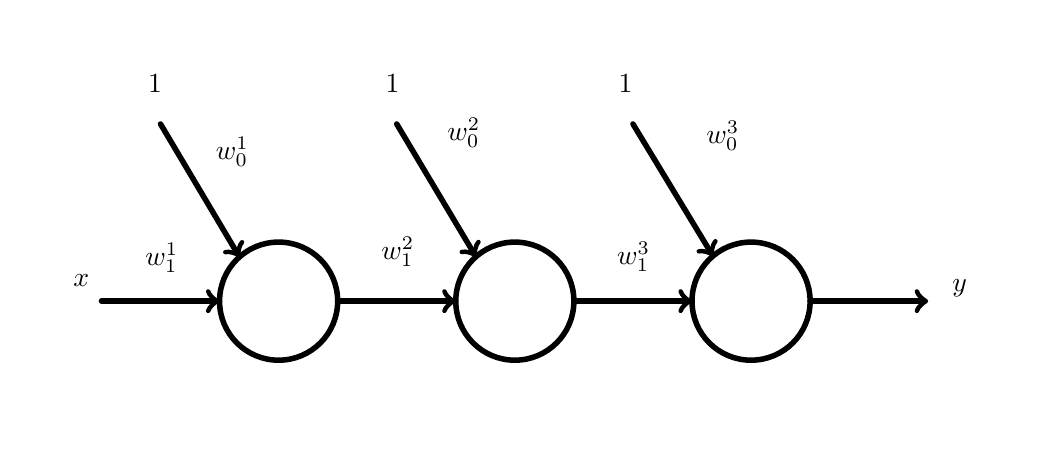
\begin{tikzpicture}[scale = 1.5, line cap=round,line join=round,x=1.0cm,y=1.0cm]
	\clip(-4.624679143882289,1.3686903642723092) rectangle (3.8521836267384844,4.8154607149701345);
	\draw [line width=2.pt] (-2.5,2.5) circle (0.5cm);
	\draw [line width=2.pt] (-0.5,2.5) circle (0.5cm);
	\draw [line width=2.pt] (1.5,2.5) circle (0.5cm);
	\draw [->,line width=2.pt] (-3.5,4.) -- (-2.831496141146421,2.874313115459547);
	\draw [->,line width=2.pt] (-4.,2.5) -- (-3.,2.5);
	\draw [->,line width=2.pt] (-2.,2.5) -- (-1.,2.5);
	\draw [->,line width=2.pt] (0.,2.5) -- (1.,2.5);
	\draw [->,line width=2.pt] (2.,2.5) -- (3.,2.5);
	\draw [->,line width=2.pt] (-1.5,4.) -- (-0.8294354120380936,2.8761280490674572);
	\draw [->,line width=2.pt] (0.5,4.) -- (1.1775032003746246,2.8820939861230355);
	\draw (-3.686865302879703,4.5) node[anchor=north west] {$1$};
	\draw (-1.67726421501702,4.5) node[anchor=north west] {$1$};
	\draw (0.2957986712481599,4.5) node[anchor=north west] {$1$};
	\draw (-4.320194130569761,2.805859627107445) node[anchor=north west] {$x$};
	\draw (3.1214195947884176,2.7693214255099416) node[anchor=north west] {$y$};
	\draw (-3.7112241039447054,3.07380643882247) node[anchor=north west] {$w_1^1$};
	\draw (-3.114433477852151,3.9750820782275555) node[anchor=north west] {$w_0^1$};
	\draw (-1.7138024166145234,3.122524040952475) node[anchor=north west] {$w_1^2$};
	\draw (-1.1535499921194723,4.13341428515007) node[anchor=north west] {$w_0^2$};
	\draw (1.0387421037307276,4.109055484085068) node[anchor=north west] {$w_0^3$};
	\draw (0.2836192707156588,3.0859858393549713) node[anchor=north west] {$w_1^3$};
	\end{tikzpicture}
\end{center} 

Как это обычно бывает, Мискузи обнаружил её в своих штанах после стирки и очень обрадовался. Теперь он хочет сделать два шага стохастического градиентного спуска, используя алгоритм обратного распространения ошибки.

У него есть два наблюдения: $x_1 = 1, x_2 = 5$, $y_1 =1$, $y_2 = 0$. Скорость обучения $\gamma = 1$. В качестве инициализации взяты единичные веса. Сначала берётся второе наблюдение, затем первое. Помогите Мискузи.

\vspace{-0.5cm}
\subsection*{[0.1] Задание 3}
\vspace{-0.5cm}

Объясните откуда взято слово из эпиграфа к работе. При сдаче работы не забудьте его произнести, иначе вы не получите баллы за третью задачу.


\end{document}